\documentclass[10pt,twocolumn,letterpaper]{article}

\usepackage{cvpr}
\usepackage{times}
\usepackage{epsfig}
\usepackage{graphicx}
\usepackage{amsmath}
\usepackage{amssymb}
\usepackage{pdfpages}

%%%%%%%%%
% Example of figure inclusion
%\begin{figure}[t]
%\begin{center}
%\fbox{\rule{0pt}{2in} \rule{0.9\linewidth}{0pt}}
%   %\includegraphics[width=0.8\linewidth]{egfigure.eps}
%\end{center}
%   \caption{Example of caption.  It is set in Roman so that mathematics
%   (always set in Roman: $B \sin A = A \sin B$) may be included without an
%   ugly clash.}
%\label{fig:long}
%\label{fig:onecol}
%\end{figure}

%%%%%%%%%
% Example table
%\noindent
%Compare the following:\\
%\begin{tabular}{ll}
% \verb'$conf_a$' &  $conf_a$ \\
% \verb'$\mathit{conf}_a$' & $\mathit{conf}_a$
%\end{tabular}\\
%
%
%
%\begin{table}
%\begin{center}
%\begin{tabular}{|l|c|}
%\hline
%Method & Frobnability \\
%\hline\hline
%Theirs & Frumpy \\
%Yours & Frobbly \\
%Ours & Makes one's heart Frob\\
%\hline
%\end{tabular}
%\end{center}
%\caption{Results.   Ours is better.}
%\end{table}

%%%%%%%%%
% another example figure
%\begin{figure*}
%\begin{center}
%\fbox{\rule{0pt}{2in} \rule{.9\linewidth}{0pt}}
%\end{center}
%   \caption{Example of a short caption, which should be centered.}
%\label{fig:short}
%\end{figure*}
%
%
%%%%%%%%%
% example citation
%   Frobnication has been trendy lately.
%   It was introduced by Alpher~\cite{Alpher02}, and subsequently developed by
%   Alpher and Fotheringham-Smythe~\cite{Alpher03}, and Alpher \etal~\cite{Alpher04}.''

    %Figure and table captions should be 9-point Roman type as in
    %Figures~\ref{fig:onecol} and~\ref{fig:short}.  Short captions should be centred.
% Include other packages here, before hyperref.

% If you comment hyperref and then uncomment it, you should delete
% egpaper.aux before re-running latex.  (Or just hit 'q' on the first latex
% run, let it finish, and you should be clear).
%
% When placing figures in \LaTeX, it's almost always best to use
% \verb+\includegraphics+, and to specify the  figure width as a multiple of
% the line width as in the example below
% {\small\begin{verbatim}
%    \usepackage[dvips]{graphicx} ...
%       \includegraphics[width=0.8\linewidth]
%           {myfile.eps}
%   \end{verbatim}
% }
%
\usepackage[breaklinks=true,bookmarks=false]{hyperref}

\cvprfinalcopy % *** Uncomment this line for the final submission

\def\cvprPaperID{****} % *** Enter the CVPR Paper ID here
\def\httilde{\mbox{\tt\raisebox{-.5ex}{\symbol{126}}}}

% Pages are numbered in submission mode, and unnumbered in camera-ready
%\ifcvprfinal\pagestyle{empty}\fi
\setcounter{page}{1}
\begin{document}

%%%%%%%%% TITLE
\title{A Predictive Model for Eye Fixations}

\author{Lauren Arnett and Chengzhi Mao\\
Columbia University in the City of New York\\
    {\tt\small \{lba2138,cm3797\}@columia.edu}
}

\maketitle

%%%%%%%%% ABSTRACT
\begin{abstract}
   Applications of tracking eye fixation location span from neuroscience and
   the study of human vision to advertising and human computer interaction. 
   We look to improve upon existing models of saliency. 

\end{abstract}

%%%%%%%%% BODY TEXT
\section{Introduction}

Please follow the steps outlined below when submitting your manuscript to
the IEEE Computer Society Press.  This style guide now has several
important modifications (for example, you are no longer warned against the
use of sticky tape to attach your artwork to the paper), so all authors
should read this new version.

%-------------------------------------------------------------------------
\section{Related Work}

\section{Dataset of Eye-Tracking Data}
\section{Learning a Model}
\subsection{Training}

\subsection{Performance}

\begin{figure*}
\begin{center}
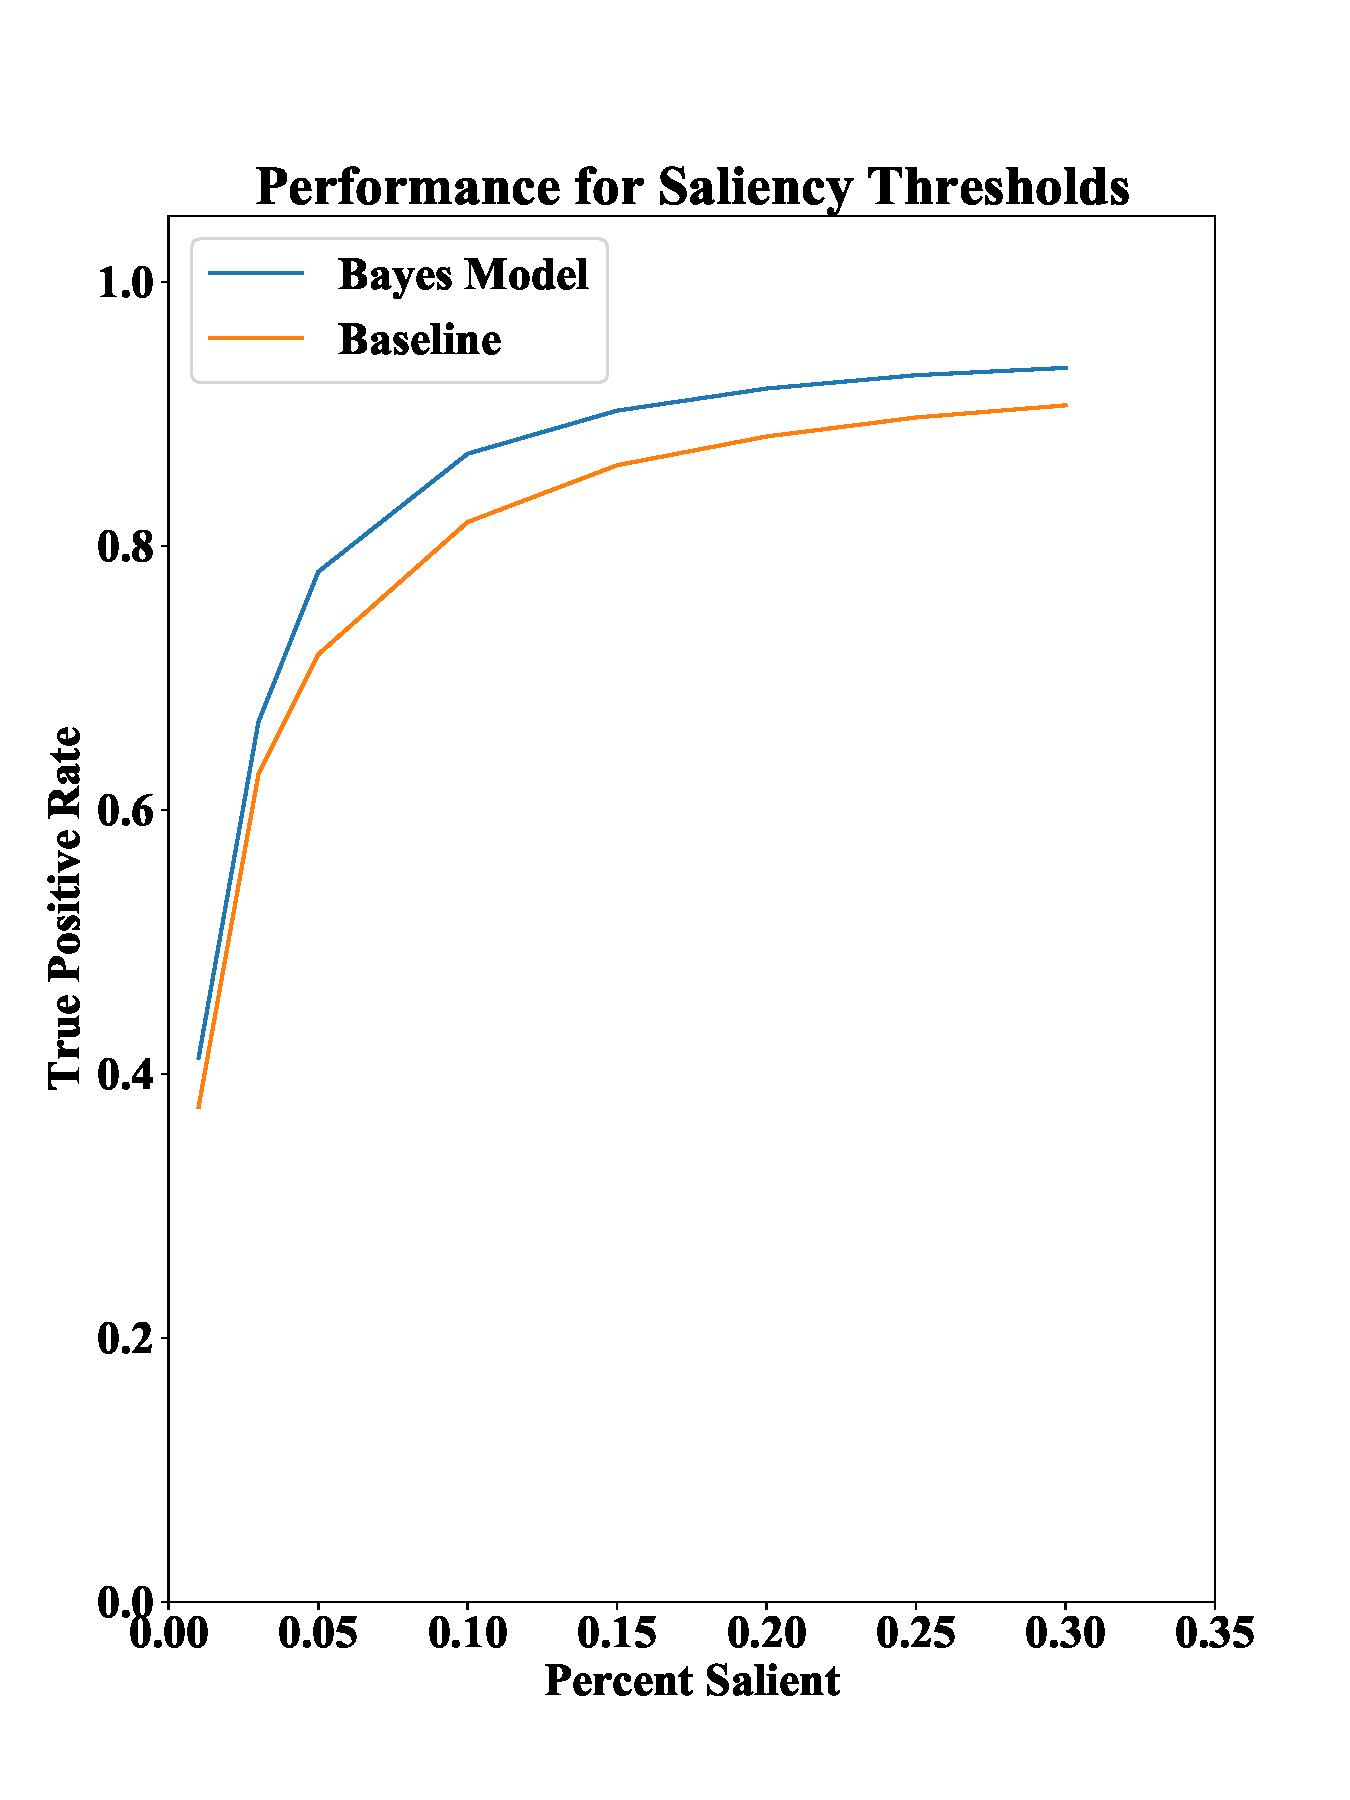
\includegraphics[width=\columnwidth]{figures/tpr.pdf}

\end{center}
   \caption{Example of a short caption, which should be centered.}
\label{fig:short}
\end{figure*}

\section{Conclusion}

%------------------------------------------------------------------------
{\small
\bibliographystyle{ieee}
\bibliography{egbib}
}

\end{document}
